\section{手工适配器实现与检查}\label{app:implementation-zh}
\path{policy_adaptation/lora_training.py} 的核心职责包括：验证输入；共享并冻结原权重；为 $A$ 使用 Kaiming-uniform 初始化、为 $B$ 使用全零初始化；实现低秩修正分支；在推理时合并权重并避免重复合并；递归替换目标线性层；统计总参数和可训练参数。

对 24 层 Qwen 模型的 CPU/float32 功能检查替换了 168 个投影层。基础模型参数为 494,032,768，新增适配器参数为 4,399,104，占合并统计总数的 0.8826\%。该检查完成前向计算和权重合并，其入口没有完整的语言模型优化循环，因此不能由它单独推断训练效果。该功能配置的 dropout 为 0.05；正式 PPO 配置为 0。

九项轻量测试分别覆盖初始等价、共享权重、非零修正公式、合并等价与幂等性、冻结基座后的优化器更新、嵌套替换和参数统计、非法输入、数据划分及只针对回答评分的本地 HTTP 接口。测试中的小型线性层实际执行了优化器更新；这与完整语言模型 PPO 实验是不同层级的证据。

\section{在线搜索记录与停止范围}\label{app:online-zh}\label{app:source-zh}
修订配置于 2026 年 10 月 31 日 12:38:01 启动。最后保存的事件时间为 13:21:18.838，工程于 13:22:05 导出，随后手动停止。以上时间均为 UTC+08:00。没有自动完成事件，不能声称完整配置预算已自动执行。

更早一次尝试保留了五个方案，但没有有效评估，其中四次已完成的代码回复为空。修订同时提高输出上限（4,096 到 32,768）并缩小搜索预算，不能把恢复归因于单一参数。保存的 Planner 记录累计 70,376 tokens，只覆盖相应记录，不代表全部任务成本。公开证据保留候选程序、配置和五次有效分数，省略包含账号界面的截图；实际在线最佳布局的原始坐标未导出，报告中的最佳布局来自独立本地执行。

源码分析固定 LLM4AD\_Next 提交为 \code{dfde353e753e9021fffe88b5b034bf0c84d90b60}，不保证托管网站与该提交完全一致。在线模型由平台报告为 \code{deepseek-v4-flash}，本文没有独立验证服务内部模型实现。

\section{历史保存失败和成功恢复}\label{app:history-zh}
早期 FP32 T4 运行完成了 512 题、32 个采样批次，但在最终保存时出现共享权重别名检查错误：
\begin{Verbatim}[fontsize=\small,breaklines=true,frame=single]
AssertionError: mismatch keys {'base_model.model.lm_head.weight'}
RuntimeError: training failed (exit 1)
\end{Verbatim}
该次运行的开发基准为 118/128，没有有效的最终适配器和训练后评估。它不能与 A10 的训练后结果配对。历史曲线来自原控制台的舍入数值，必须与 A10 的精确事件记录分别解释。

\begin{center}
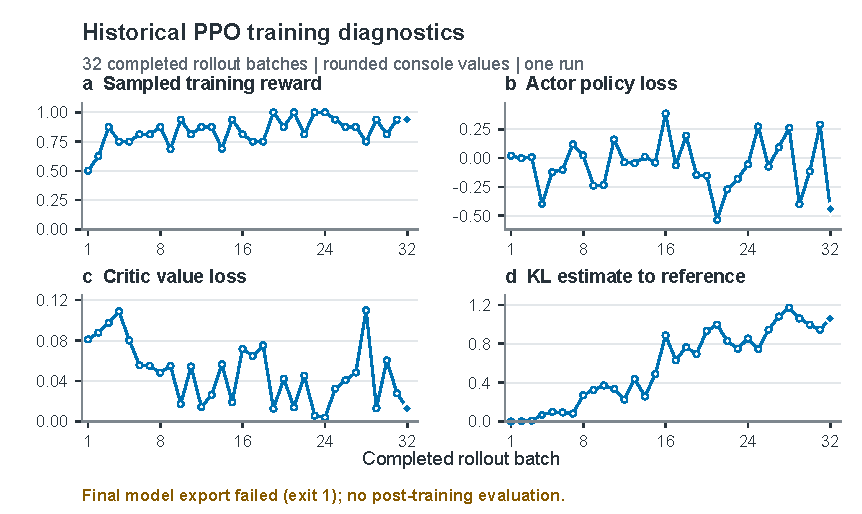
\includegraphics[width=146mm]{../../figures/observed_attempt.pdf}
\end{center}
\figcaption{fig:historical-zh}{早期 T4 的历史训练诊断。32 批计算完成后仍发生最终保存失败；曲线不能代替保存和重载证据，也不代表后来 A10 的结果。}

保存修复仅在输出层权重与输入嵌入是同一个 Parameter 时接受缺失的别名，真正缺少独立权重仍会报错。另一个采样器修复补齐 \code{pad\_len=None}。最终采用单 GPU eager attention 路径，关闭 packing 和 ring attention，并对固定源码做哈希检查后延迟三个未使用的 ring 操作导入。它不模拟 FlashAttention 的计算，若调用真实 ring 操作仍要求安装该依赖。

环境元数据保留了一项已声明的例外：OpenRLHF 0.6.0 要求 FlashAttention，但它未安装。真实 CUDA Actor/Critic 前向、反向和 FusedAdam 参数更新通过后，又通过独立 16 题的保存及 Actor 重载检查，再从原始基座开始完整运行。成功环境为 Python 3.10、PyTorch 2.5.1+cu124、Transformers 4.48.3、PEFT 0.14.0、DeepSpeed 0.16.3、Ray 2.42.0。PPO 显式使用 eager；原评估函数可能使用 SDPA。

成功运行于 2026 年 11 月 8 日 09:48:14 UTC 完成。约九秒后另一调用因已有受保护产物而被拒绝，其导出清单因而记录后一次调用失败。它不推翻前一次的退出码 0、完整 32 批指标、有限且非零的适配器、Actor 实际重载和逐题回答。原始本地导出单独保留；公开版本仅整理便携证据子集。Critic 只检查了权重，没有独立重载，也没有完整的 PPO 优化器恢复检查点。

\section{复现材料的阅读顺序}\label{app:reproduction-zh}
先阅读 \path{policy_adaptation/results/} 中训练前后的逐题回答和采样指标，再对照训练配置、适配器检查和模型修订。历史 T4 保存失败的指标必须单独阅读。\path{program_search/} 中的在线评估 CSV 与本地保存坐标是两种记录，不能互相替代。

\path{policy_adaptation/} 提供手工 LoRA、固定参数训练入口、奖励服务、共同评估函数和兼容修复；\path{program_search/} 提供最佳导出构造程序和几何检查。公开副本只规范身份信息和特定机器路径，不改变实验数值或适配器权重。绘图入口读取保存数据，不发起训练或在线搜索；本地重新执行构造程序则会产生新的本地计算记录，数值可能随库版本变化。

全新环境安装脚本是整理后的复现方案，尚未在另一台干净 GPU 机器上重复完整实验。免费 GPU、网络与外部模型服务可用性仍是外部条件。依赖安装、基础检查和显式训练命令见仓库中英文说明；轻量检查不等于重新完成 PPO 或托管搜索。
